\chapter{Introduction}

This is \verd, a library for evaluating the geometric qualities of regions of space.
These regions of space are typically those used as problem domains for partial differential equations,
and are typically partitioned into subregions known as finite elements, finite volumes, or boundary elements.
Subregions are typically simple shapes defined by a few vertices.
The subregion shapes \verd\ currently supports include triangles, quadrilaterals, tetrahedra, and hexahedra.

\section{Measuring Quality with Metrics}

\verd\ evaluates geometric qualities on a subregion of the partition with metrics.
A metric is a real number that may be assigned to the subregion.
Some metrics, which we will call \textbf{proper metrics}, are normalized so that
their values are $1$ for ideally-shaped subregions and
their values tend to $\infty$ for ill-defined, poor quality, or degenerate subregions.
Examples where a proper metric should tend to $\infty$ include non-planar quadrilaterals,
triangles with edges of vastly different lengths, and subregions with coincident vertices.

\section{History of \verd}

\verd\ has its first roots in the \href{http://www.cs.sandia.gov/capabilities/VerdeMeshVerificationSuite/index.html}{\verde}\footnote{\href{http://www.cs.sandia.gov/capabilities/VerdeMeshVerificationSuite/index.html}%
           {\texttt{http://www.cs.sandia.gov/capabilities/VerdeMeshVerificationSuite/index.html}}} project.
\verde\ is a simple program to
read Exodus meshes, and analyze them for possible problems.  Quality was one of
the areas of analysis that \verde\ covers.  It was realized that \verde\  and 
\href{http://cubit.sandia.gov/}{\cubit}\footnote{\href{http://cubit.sandia.gov/}{\texttt{http://cubit.sandia.gov/}}} did not yield the same results when analyzing the geometric qualities of meshes.
As a result, \verd\ was created so that both \verde\ and \cubit\ could share the same
code and produce the same results.  \verd\ also has roots in the \cubit\ project
and many other contributors, both theoretical and practical.
\verd\ was initially licensed under the LGPL.

Meanwhile, the \href{http://www.vtk.org/}{Visualization Tool Kit
(\vtk)\footnote{\href{http://www.vtk.org/}{\texttt{http://www.vtk.org/}}}} did not 
have any support for general purpose mesh quality assessment (with the
exception of a method to calculate the tetrahedral radius ratio,
written by Leila Baghdadi, Hanif Ladak, and David Steinman at the
Imaging Research Labs, Robarts Research Institute). Due to the need for
such a tool, and because Kitware was unwilling at that time to
include LGPL libraries in the \vtk\ repository, Philippe
P\'ebay and David Thompson generalized the \href{http://www.vtk.org/doc/nightly/html/classvtkMeshQuality.html}{\texttt{vtkMeshQuality}}\footnote{\href{http://www.vtk.org/doc/nightly/html/classvtkMeshQuality.html}%
                 {\texttt{http://www.vtk.org/doc/nightly/html/classvtkMeshQuality.html}}}
filter in 2004 to compute one or more measures of geometric quality for each 2-D
and 3-D cell (triangle, quadrilateral, tetrahedron, or hexahedron) of
a mesh for a variety of metrics.
In addition to computing per-element qualities, methods to compute their average, minimum, maximum,
and variance over the entire mesh where also added.
These descriptive statistics are stored in the output mesh's \textsc{FieldData}. This filter allows forx
further processing and/or visualization of the per-element quality,
for instance using
\href{http://www.paraview.org/}{\PV\footnote{\href{http://www.vtk.org/}{\texttt{http://www.paraview.org/}}}}
as illustrated in Figure~\ref{f:viz-qual}
%%%%%%%%%%%%%%%%%%%%%%%%%%%%%%%%%%%%
\begin{figure}[ht]
\begin{center}
\hfil
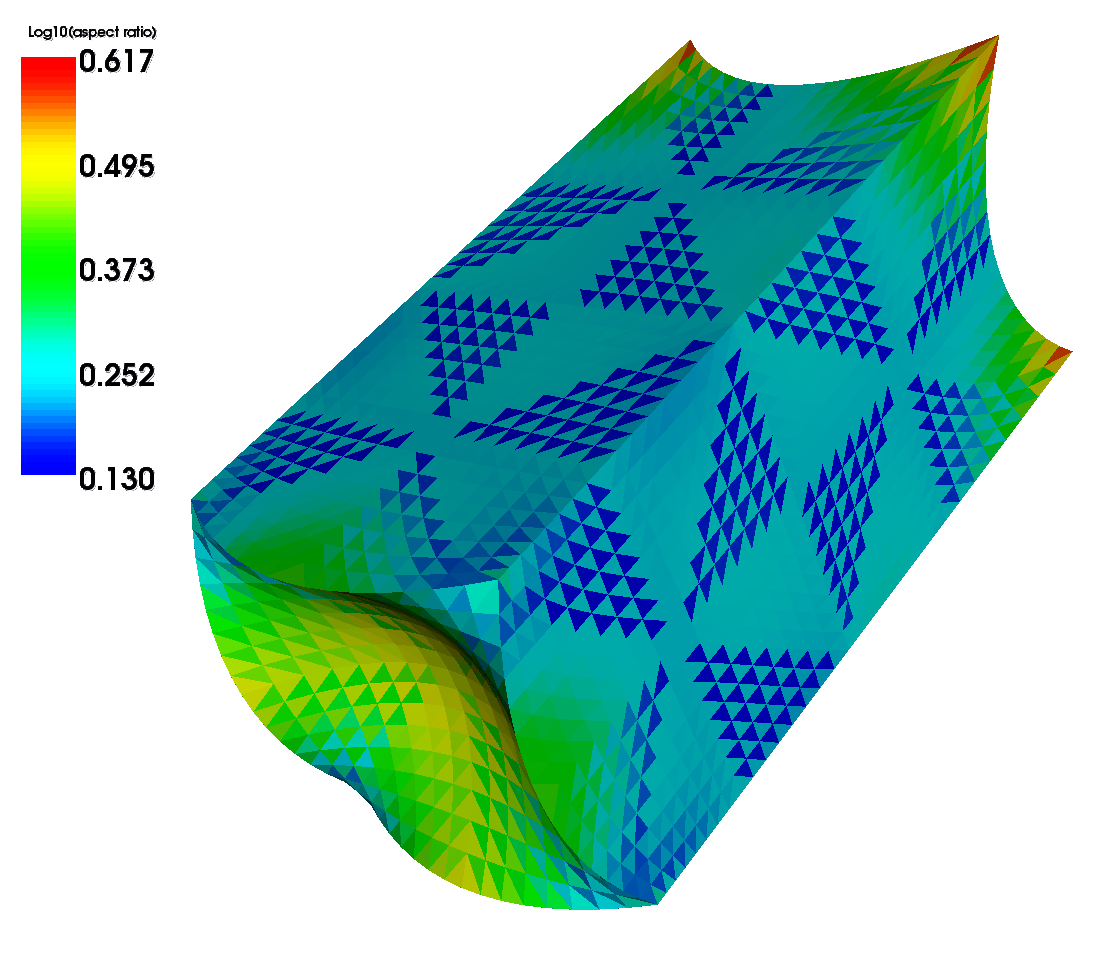
\includegraphics[height=4.5cm]{quality-streamingTess}
\hfil
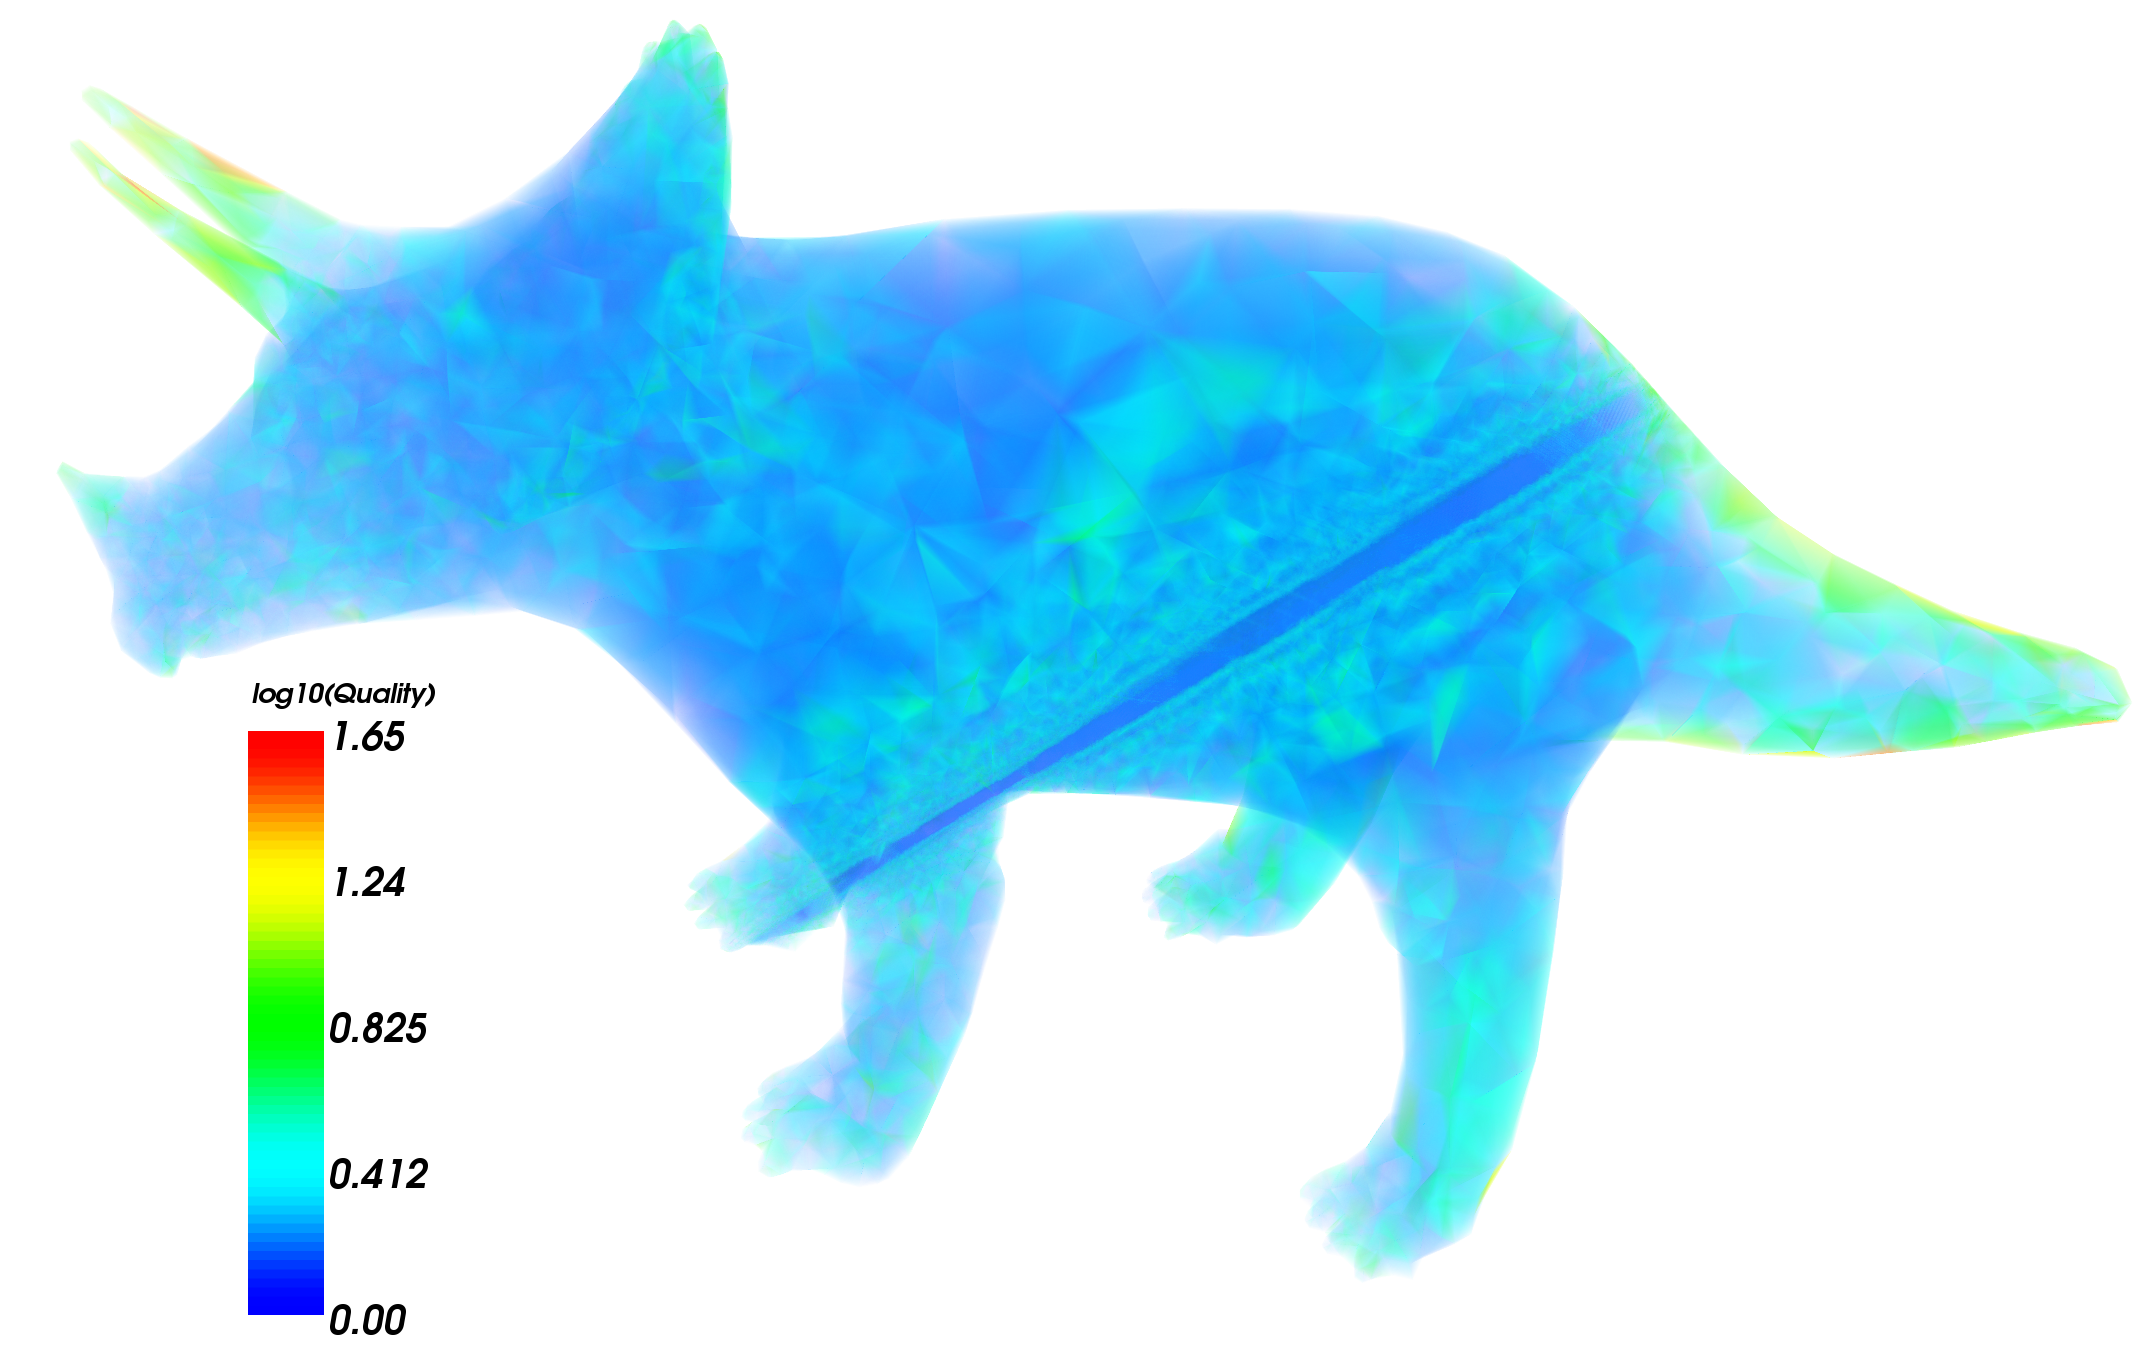
\includegraphics[height=4.5cm]{tri4qualVR-bq2}
\hfil
\caption{\label{f:viz-qual} Surface (left) and volume (right)
renderings with \PV\ of the per-element base-$10$ logarithms of the
aspect ratios for two tetrahedral meshes.} 
\end{center}
\end{figure}
%%%%%%%%%%%%%%%%%%%%%%%%%%%%%%%%%%%%

Following a change in \verd's licensing scheme, from the LGPL to a modified BSD-style license,
it was decided in late 2006 to use \verd\ in \vtk\ for the same reasons that \verd\ was initially
created, by:
\begin{enumerate}
\item 
moving all metric implementations from \texttt{vtkMeshQuality} to
\verd\, while retaining the best implementation when the same metric
was implemented in both software packages;
\item
using \texttt{vtkMeshQuality} as a wrapper around \verd{}; and
\item
\label{item:API-changes}
resolving naming inconsistencies and redundancies.
\end{enumerate}
It is important to former \verd\ users to note that
item~\ref{item:API-changes} has resulted in changes to \verd{}s API,
although efforts have been made to preserve backwards-compatibility
as often as possible; this document underscores these modifications.

\section{Organization}

After this introduction, the document can be broadly divided into sections covering
first the practical aspects and
second the theoretical aspects of geometric quality evaluation.
In these sections:
\begin{itemize}
\item Instructions on the practical aspects of obtaining, building, and installing the library are described.
\item Notes on the application programming interface (API) are provided.
\item A summary of each metric is provided, sorted first by the shape of the subregion they deal with and then by name.
\end{itemize}

The summaries in the last section form the bulk of the document and
each contains a mathematical description of its quality metric $q$.
In addition to a formula for each metric, information on the typical, acceptable, and total range
of values taken on are presented in a tabular form according to the conventions outlined below in \S\ref{s:metric-range}.
Each summary table also contains a note on the dimension of its metric -- where we use
dimension in terms of the units associated with each metric value.
Proper metrics have no dimension (which is denoted with a $1$) but some metrics
such as area, volume, or maximum angle do have dimension.
We use $L$ to denote dimensions of length and $A$ to denote dimensions of angle.
When a metric has a dimension repeated, an exponent is used to show the count.
For example, volume has 3 length dimensions and would be denoted $L^3$.
While the precise units of length depend on the input coordinates,
angles are always reported in degrees.
The summary table also contains an entry for the value that the metric takes on for some
ideally-shaped subregion, when the metric is shape-invariant (unlike,
\emph{e.g.} volume metrics which are not preserved by scaling). For
triangular, quadrilateral, tetrahedral, and hexahedral shapes, this is
respectively an equilateral triangle, a square, a regular tetrahedron,
and a cube. For proper metrics, this value will be $q = 1$.
Finally, each summary table has a reference to a book or paper where its metric is defined and discussed.
If no reference is listed, the metric is one that is traditionally used but not present
in the literature we are aware of.

Where possible, notes on the intended use of the metric are included.
\verd\ provides a variety of metrics for each subregion shape it supports.
Since a metric is a single real number, it cannot completely describe the shape of its corresponding subregion.
Thus, most metrics are used to identify a single type of problem with a subregion's shape.
Because many numerical techniques are used to solve partial differential equations,
the best metric to characterize the geometric quality of a region will vary.

\section{Metric Ranges\label{s:metric-range}}

Each metric may take on any value on the real number line, but typically subsets of this range
are of interest since values for misbehaved or geometrically degenerate elements are often used to
segregate or eliminate elements.
The summary tables provided for each metric include three intervals on the real number line:
\begin{center}
\begin{tabular}{r@{ : }p{3.2in}}\hline
Acceptable Range&Well-behaved elements will have metrics in this range.\\
Normal Range    &All elements except those with degeneracies will have metrics in this range.\\
Full Range      &All elements including degenerate ones will have metrics in this range.\\ \hline
\end{tabular}
\end{center}

\section{Metric Behavior}

The metrics in this report are all checked for overflow like so:
\begin{algorithmic}[1]
\STATE Given a double-precision quality metric value $q$,
\IF{$q > 0$}
\STATE $q\gets\min\left( q, DBL\_MAX \right)$
\ELSE
\STATE $q\gets\max\left( q, -DBL\_MAX \right)$
\ENDIF
\end{algorithmic}

Where applicable, the metrics in \verd\ were verified against theory for:
\begin{itemize}
\item Node order invariance.
\item Continous solutions within the normal range.
\end{itemize}
